%%%%%%%%%%%%%%%%%%%%%%%%%%%%%%%%%%%%%
%% Master Thesis - Computer Engineering
%% Copyright 2009 Ricardo Alexandre Fiorelli, Erick Poletto
%% This document is distributed by the terms of the license
%% included in the file LICENCE.
%%%%%%%%%%%%%%%%%%%%%%%%%%%%%%%%%%%%%

%%%%%%%%%%%%%%%%%%%%%%%%%%%%%%%%%%%%%
%% Third Chapter
%% Methodology
%%%%%%%%%%%%%%%%%%%%%%%%%%%%%%%%%%%%%

\chapter{Methodology} \label{chap3:methodology}

   This chapter will describe the steps taken to the end of constructing the components database and of validating the data contained in it.
These can be shortly described as follows:
    \begin{description}
        \item[Phase 0: Project definition -] As this work is part of a project aimed to create a methodology to implement a Green ICT strategy, this first phase consisted of the definition of the logical components of this project and of how the current work would collaborate to it;
        \item[Phase 1: Analysis of Benchmarking Softwares -] A number of existing softwares were analysed and those that have proven to be more adequate were selected. A list of the analysed softwares can be found in Appendix~\ref{app:list_other_energy_management_tools};
        \item[Phase 2: Catalog -] The tools were used to obtain information about computer components that were later used to create a component database;
        \item[Phase 3: Database design and construction -] The database schema was designed and data began to be inserted into the relations;
        \item[Phase 4: Analysis -] The validity of the stored data was tested with the help of direct measurements.
    \end{description}


\section{Overview} \label{sec3:overview}
    The main and broader objective of the research that is being conducted is to develop a methodology to implement a green ICT strategy. Namely, the methodology would provide a set of tools to guide the hardware acquisition process in an organization either in terms of workstations or of datacenter equipment. The present work will contribute to this research by providing a component database with information related to hardware components, which will be used as one of the inputs of the methodology. This work was conducted in order to determine how much energy a computer's components, for instance, CPU\footnote{Central Processing Unit}, Memory and Hard Drives spend and also how much they would affect the cost of acquisition of new computers as a whole. This is calculable with information such as component performance, power consumption and price. The analysis was carried out with the help of specialized softwares that will be described in the following sections and also with analytical measures made with an energy measurement device. In the end the benchmarking measures obtained from these softwares were compared with both the measures obtained from the device and with information provided by the component datasheets. With the benchmarking software, more than 1000 components were categorized in a database, whose schema can be found in Figure~\ref{fig:database_schema}. Firstly, the SiSoft Sandra's database~\ref{sec3:sandra} was used to collect the components and separate them by categories, along with their benchmark related data. Secondly, WebSPHINX~\ref{sec3:websphinx} was used to create a collection of components and their respective MPNs. In the end, an energy measurement device~\ref{sec3:energy_measurement_instrument} was used for the comparison and validation of the results given by the other benchmarks and acquisition of new data. 
    Finally, these data were all linked in a database for later comparison. 

\section{Research Design} \label{sec3:research_design} 
    The experimental method of research was used in this study. Figure~\ref{fig:experimental_method_approach} draws the steps of the method. To define the experimental type of research, Bryman \cite{bryman89} states that ``the experimental design (\ldots) allows the causal hypothesis that underpins the question to be examined'', which means that this method is a systematic and scientific approach to research in which the researcher manipulates one or more variables, controlling and measuring any changes in other variables. The emphasis given is on the results and analysis of the benchmarks provided and their measures. It allows to verify the thesis on which this work is based by making use of empirical methods which in the case relates to the benchmarks used.
    \begin{figure}[htbp]
        \centering
            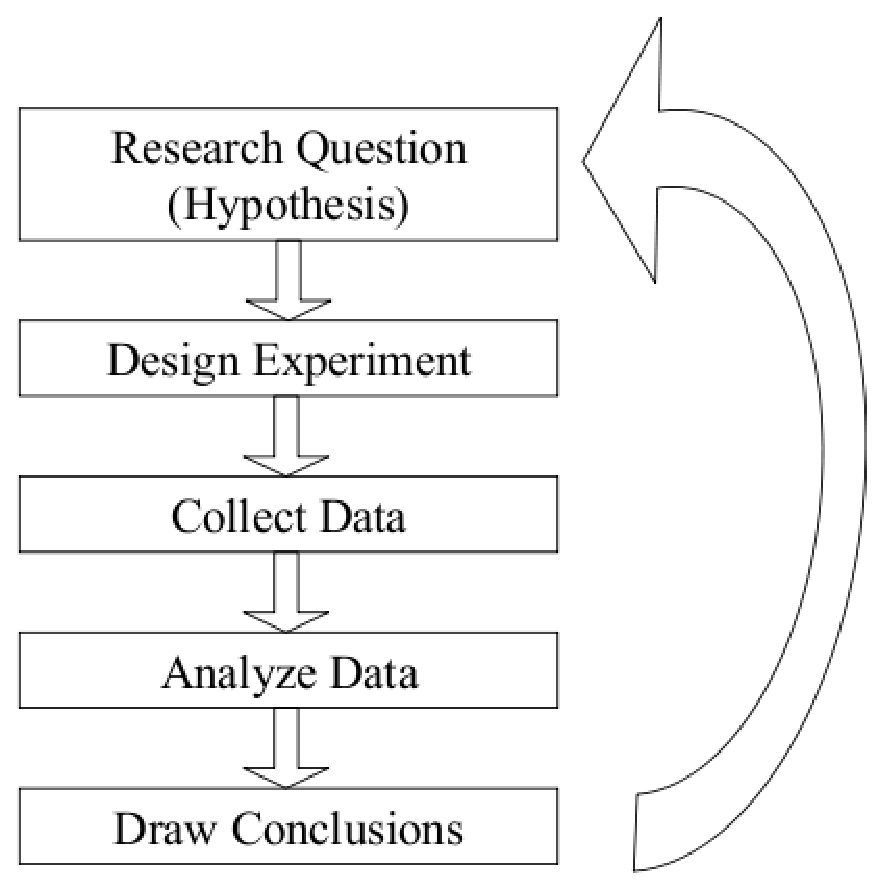
\includegraphics[scale=0.5]{graphics/experimental_method_approach}
            \caption{The Experimental Design Process}
            \label{fig:experimental_method_approach}
    \end{figure}

    % explicacao da figura
    %/********* Os proximos paragraphs foram criados para direcionar o pensamento e deve ser mantidos como comentario*******/
    %    \item[Universe o Study] (whether a tribe, or a village, or an urban areas, or a particular group, etc.) - no nosso caso, os componentes do computador e o data center
    The present study is meant to identify the power consumption of the computer components and to evaluate the accuracy of the obtained data through direct measurements. The quantitative method (direct measurements and benchmarking), other than the qualitative method, was employed in order to identify the more energy efficient components that may be used in green datacenters. Among all components, the ones included in the measurements are: Chipsets, Memory, Data Storage, Processor and the chassis (fan, power supply, etc).
    %    \item[Subject of Study] (whether it focuses on the whole society, or any specific institution or a part of it).
    The choice of analysing each component separately and also the whole computer power consumption was made in order to evaluate the behaviour of a machine configuration where a number of components have to interact and confront it to the expected behaviour of each component.
    %    \item[Relationship Between certain variables] (Formulating a Research Design but it is not obligatory to start with a Research Design).

    %    \item[Set of selected methods for obtain data] (whether participant observation, Interview, Questionnaire, or some other methods of data collection would be used).
    In order to obtain relevant data, three analysis' methods were used: empirical, benchmarking and research. For the empirical method, it was used an energy measurement device (section~\ref{sec3:energy_measurement_instrument}) that connected the electrical plug to the computer, and the measure was written in a spreadsheet~\ref{tab:toolino_table}. While doing this, the benchmarking tool (section~\ref{sec3:sandra}) was performed in the host computer in order to acquire measures in a set of different situations. The last method, the research, carried with the use of a web crawler called WebSPHINX, provided information about the price and the MPN of each component in the database. As each component has a unique MPN this made possible to uniquely identify each one of them, enabling thus the use of a normalized database over the identified components.

    %    \item[Analytical Categories] (by which the empirical data is subjected to analysis and interpretation).
    In a later stage, all the data acquired by the measurement approaches was separated by categories and components. The database generated is described and furtherly explained in the section~\ref{sec3:data_processing_analysis}.
    
\section{Energy Management and Benchmarking Tools} \label{sec3:energy_management_tools}
    In order to obtain relevant information about the data required for making the comparison between the components, some energy management and benchmarking tools were used.
    
    The softwares that used were selected over the other available ones for their superior evaluation on the following criteria:
\begin{description}
    \item[Size of Database] The database of components used by the software, in order to get a good result, should be considerably large;
    \item[Characteristics of Benchmarks] The benchmarks provided by the software should provide information about the energy consumed for each component;
    \item[Number of Benchmarks] The software should have a good variety of benchmarks;
    \item[Quality of Benchmarks] Although the number of benchmarks should be sufficient in number, the quality, precision and relevancy were also important in the decision method;
    \item[Ease of Use] In the sense that the software should provide an ambient of work that is both intuitive and user-friendly;
\end{description}
    
    The acquisition of data was made analysing the results of these benchmarks, making use of their database and system measurement capabilities.

    \subsection{SiSoftware SANDRA} \label{sec3:sandra}

    SiSoftware Sandra\footnote{The \textbf{S}ystem \textbf{AN}alyser, \textbf{D}iagnostic and \textbf{R}eporting \textbf{A}ssistant} is an information and diagnostic utility. It provides most of the information one need to know about their hardware, software and other devices whether hardware or software. SANDRA was the main software utilized to benchmark the data in this thesis work. It contains a vast database of components associated with both benchmark results and manufacturer specifications.
    
    This software gives the possibility of benchmarking computer devices at several levels of operation. For example, it can benchmark a processor and show its performance over several operational levels, from power saving to full workload. Moreover, it may monitor the performance in several levels, from the overall performance of a system to the performance of its components, including CPU, memory, hard disks, CD/DVD ROM, network adapters, etc. For that reason, it is considered one of the most complete benchmarking tools available. Besides the benchmarking, Sandra also provides hardware specifications for components such as the Motherboard, processor, disks, printers, etc. One last resource is the benchmarking of software performance, which is provided for key softwares (web browsers, e-mail program, etc.), OS information, processes, memory usage and more.
    
    The detailed list of modules utilized by SiSoftware Sandra can be found in Appendix~\ref{app:sandra_modules}.
    
    Furthermore, SiSoftware Sandra provides a catalogue of pricing, which, in addition to the power consumption and other important characteristics, enables the user to choose the best combination (which means the maximum performance/power ratio) of devices can be chosen to the server.
    
    \subsection{Energy Measurement Instrument} \label{sec3:energy_measurement_instrument}

        \begin{figure}[htbp]
            \centering
                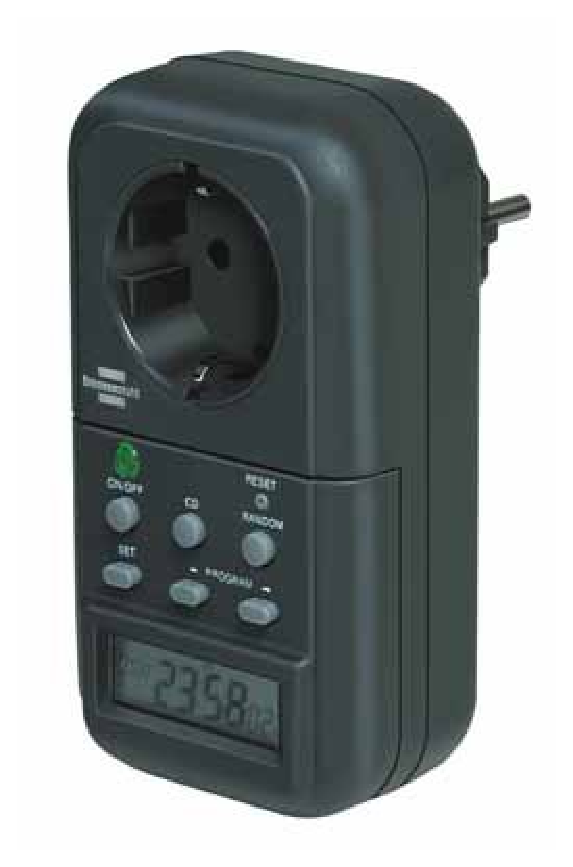
\includegraphics[scale=0.6]{graphics/energy_measurement_instrument}
                \caption{Energy Measurement Instrument}
                \label{fig:energy_measurement_instrument}
        \end{figure}
        The device, which can be seen on Figure~\ref{fig:energy_measurement_instrument}, was used for comparing and validating the results of the benchmarks given by Sandra. After the result of the benchmark was obtained from the SiSoftware Sandra, this equipment that was connected to the computer read how much energy it was consuming. The data from both sources were inserted in the database.
        
    \subsection{WebSPHINX - A Personal, Customized Web Crawler} \label{sec3:websphinx}
        WebSPHINX\footnote{Website-Specific Processors for HTML Information Extraction} is a Java class library used for web crawling. It provides a way to browse and process web pages automatically.
        
        This piece of software was used to determine the component´s MPN code and also to create the pricing list, used in the database described in~\ref{sec4:analysis}.

        The target website used to obtain the information\footnote{http://www.sisoftware.net/} provided a specific search engine for each kind of component. The searches for each one of those used a base URL concatenated with a page number and the result pages were standardised and presented a list of components of a specific category (i.e. hard drives or processors) along their MPN number and suggested price. This made possible the automation of the search and the subsequent filtering of the desired information.
        The individual components along with their MPN codes were inserted in the Device relation in the database while the pricing data were used in the Price relation.

    \subsection{CPU-Z} \label{sec3:cpu-z}
        CPU-Z detects information about the CPU, RAM Memory, motherboard, chip-set and more. That program was used to complete the database with missing information about the components.

        This software extracts system information such as name, number of cores, cache size and clock frequency for processors; mainboard model and chipset and size, bandwidth and type for main memory. This information is particularly useful when SiSoftware Sandra cannot identify a component or individuate its power consumption. The data obtained with the use of CPU-Z is confronted with the power consumption of similar components to obtain an estimate of the desired value.

\section{Data Processing and Analysis} \label{sec3:data_processing_analysis}
    % TODO
    % explicar sobre a tabela geralzona que linka todos os componentes.
    % se nao colocar aqui, mudar para o capitulo 4. Só não trocar o label ---- melhor escrever no 4o capitulo. o database schema eh um resultado do trabalho
    
    \subsection{Measures}\label{sec3:measures}
        For each computer in which this method of data acquisition was performed the results were inserted in the tables~\ref{tab:toolino_sandra_table} and~\ref{tab:toolino_table}. The Table~\ref{tab:toolino_sandra_table} was obtained by running SANDRA benchmarks where the first column ``Processor Benchmark'' represents the results from the ``Processor Arithmetic'' benchmark, where the energy spent by the processor is displayed in the results. Afterwards, the ``Cache \& Memory'' benchmark was executed and its estimate of the power consumption of processor, chipset and memory was inserted in the table.
        
        Similarly, for the measurement device (table~\ref{tab:toolino_table}) the power consumption was measured in three situations: firstly, with the computer in idle state (monitor on, with no user processes running). Secondly, with the same configuration but with the monitor powered off. Lastly, the power consumption was measured with the processor fully stressed, i.e. while running SANDRA performance benchmarks. One limitation we had while taking measures is that it was only possible to obtain data from notebooks. In this way the difference between the measures with the monitor turned on or off should provide the monitor power, which is not considered by the Sandra benchmarks.
        
        In order illustrate an example of the acquired data, only a few measures are displayed in the tables. The full version is evinced in Appendix~\ref{app:measures_toolino}.
    \begin{table}[htbp]
        \centering 
        \begin{tabular}{|c|c|c|}        \hline
        Computer & Processor & Cache \& Memory \tn
        Model & Benchmark (W) & Benchmark (W) \tnhl
        HPdv3500el (13.3'') & 19.69 & 26.69 \tnhl
        HPdv6580el (15.4'') & 32.01 & 40.06 \tnhl
        Compaq-nx9420 (17.0'') & 26.93 & 36.16 \tnhl
        Acer Aspire 4720z (15.0'') & 19.78 & 34.57 \tnhl
        Acer Aspire 5930G (15.4'') & 25.13 & 32.13 \tnhl
        \end{tabular}
        \caption{SANDRA Table Analysis}
        \label{tab:toolino_sandra_table}
    \end{table}
    \begin{table}[htbp]
        \centering \resizebox{\textwidth}{!}{ % Fazendo a tabela caber no espaco da pagina
        \begin{tabular}{|c|c|c|c|c|}        \hline
        Computer & Idle with & Idle with  & Estimated Monitor & Processor \tn
        Model & Monitor On (W) & Monitor Off (W) &  Power (W) & Fully Stressed (W) \tnhl
        HPdv3500el (13.3'') & 28.57 & 25.19 & 3.38 & 35.64 \tnhl
        HPdv6580el (15.4'') & 62.18 & 57.14 & 5.04 & 85.27 \tnhl
        Compaq-nx9420 (17.0'') & 78.89 & 74.65 & 4.24 & 79.64 \tnhl
        Acer Aspire 4720z (15.0'') & 44.57 & 39.88 & 4.69 & 67.28 \tnhl
        Acer Aspire 5930G (15.4'') & 44.48 & 39.56 & 4.92 & 62.83 \tnhl
        \end{tabular}}
        \caption{Energy Measurement Device Table Analysis}
        \label{tab:toolino_table}
    \end{table}
    %XXX nao se eh cabivel explicar algo aqui ou deixamos para o proximo capitulo
    
    \subsection{Components Database}\label{sec3:components_database}
        % aquele gerado pelo access do SANDRA
        The Sisoftware SANDRA has a database with the results of all benchmarks for a considerable number of components making it proper for component comparison in terms of performance and energy efficiency. The data from this database was extracted to fit the database described in Appendix~\ref{app:sandra_benchmark_table_schema}.
        
        The only issue related to the SANDRA database is the that components are not treated uniquely and each benchmark has its own list of components. For example, a benchmark of cryptography for the processor provides just the processor family ``Intel Core 2 Duo T8400'' while other relations may store a specific processor model, such as ``Intel Core Duo T2300 (DC, 1.66GHz, 2MB L2)''. As the database cannot be normalized in this way, it was necessary to provide an unique code for each component.
        
        In Sisoftware website there exists a list of components and their suggested price. This list has a web-based version and also can be accessed inside the software, which besides the price provides all the information present in the linked inside the software for each component that is being analysed. An information from the website that has proven to be useful is the MPN code, that, like the ISBN for books, is unique for each component. Therefore, in order to create a unique relation with all the components that would be referred by the benchmark relations it was necessary to obtain these MPNs and assign them to the components and afterwards link them to the specific benchmarks. An example of the table generated with WebSPHINX for processors are shown in Table~\ref{tab:example_table_websphinx}.
                
        \begin{table}[h!tb]
            \centering
            \begin{tabular}{|c|c|}
            \hline
            \textbf{Processors} & \textbf{MPN} \tnhl
            AMD Phenom II X4 940 Quad Core Processor & HDZ940XCGIBOX \tnhl
            Intel Core 2 Duo E8400 Dual Core Processor & BX80570E8400 \tnhl
            AMD Athlon 64 X2 Dual Core Processor & AD775ZWCGHBOX \tnhl
            AMD Phenom II X3 720 Triple Core Processor & HDZ720WFGIBOX \tnhl
            Intel Core 2 Q9550 Quad Core Processor & BX80569Q9550 \tnhl
            \end{tabular}
            \caption{Example of Table Generated by WebSPHINX}
            \label{tab:example_table_websphinx}
        \end{table}
        
    \subsection{Manufacturer Specifications}\label{sec3:manufacturer_specifications}
        The last set of information that was required by the final evaluation were the manufacturer specifications. These data were obtained by searching for each analysed computer model in the manufacturer site and looking for its components. As the more power-consuming components in a computer (excluding power supply components) are the processor, mainboard and memory, these were identified in the manufacturer site.
        After identifying the processor, mainboard and memory used in each computer, their specifications were used to validate the informations obtained by the benchmarks.
        
        
        
